\chapter{Teilchen, Wellen und die Auflösungsenergie}

\section{Teilchen oder Felder?}

Worum geht es in der Teilchenphysik? Um Teilchen---, doch diese Antwort wirft sofort eine uralte Frage auf: Ist die Natur diskret? Diskret bedeutet hier, dass Materie aus getrennten, unteilbaren Einheiten besteht, nicht, dass sie taktvoll ist. Das griechische Wort \emph{Atom} bedeutet unteilbar, obwohl sich die Gegenstände, die heute Atome genannt werden, zerlegen lassen. Vorerst verwenden wir \emph{Teilchen} als allgemeine Bezeichnung für eine diskrete Einheit.

Das entgegengesetzte Bild ist ein Kontinuum. Materie besteht dann nicht aus getrennten Stücken, sondern ist kontinuierlich im Raum verteilt. Ihre natürliche Sprache ist die Sprache der Felder. Ein Feld ist eine Funktion des Ortes: Die Dichte eines Materials ist ein Feld, und auch das elektrische und das magnetische Feld sind Felder. Letztere bestimmen, wie sich geladene Teilchen bewegen; klassisch stellt man sich die Felder selbst jedoch als kontinuierlich im Raum verteilt vor.

Die historische Reihenfolge dieser Ideen sollte man nicht überbewerten. Die Abfolge ist hilfreich, weil sie die Logik der Argumentation verdeutlicht, nicht weil sie eine verlässliche Chronologie liefert. Zum Vokabular der Teilchen gehören Atome, Moleküle, Stöße und lokalisierte Objekte; zum Vokabular des Kontinuums gehören Felder und kontinuierlich veränderliche Eigenschaften. Welches Bild ist richtig? Die Quantenmechanik verhindert, dass eines von beiden vollständig richtig ist, aber ebenso, dass eines vollständig falsch ist.

Die Darstellung wird teilweise in sich abgeschlossen sein, auch wenn spätere Argumente auf Quantenmechanik, klassische Mechanik, spezielle Relativitätstheorie und Elektromagnetismus zurückgreifen. Die unmittelbare Frage ist einfacher: Was überzeugte die Menschen zunächst davon, dass Materie tatsächlich diskret ist?

\section{Chemische Hinweise auf diskrete Materie}

Die ersten überzeugenden Hinweise kamen, zumindest in dieser logisch aufgebauten Darstellung, aus der Chemie und nicht aus der Physik. Diese Unterscheidung ist künstlich: Chemie ist weitgehend die Physik der Atome und Moleküle. Dalton verglich die Massen gleicher Molekülzahlen verschiedener Stoffe. Festzustellen, dass die Proben tatsächlich gleich viele Moleküle enthielten, war selbst ein großes Problem. Hier kommt Avogadros Name ins Spiel: Ein Mol enthält so viele Moleküle wie die Avogadro-Zahl angibt. Um Proben mit gleicher Molekülzahl miteinander zu vergleichen, musste man den konkreten Wert dieser Zahl nicht kennen.

Das auffällige Muster bestand darin, dass die molaren Massen ungefähr ganzzahlige Vielfache der molaren Masse von Wasserstoff waren. Die Faktoren waren im Allgemeinen weder \(3/2\) noch \(\pi\) noch beliebige reelle Zahlen, sondern Zahlen nahe bei ganzen Zahlen. Kohlenstoff-12 besitzt beispielsweise ungefähr zwölf der Masseneinheiten, die durch Wasserstoff repräsentiert werden. Das deutet stark darauf hin, dass die Materie aus wiederholt vorkommenden Bausteinen nahezu gleicher Masse aufgebaut ist.

Die moderne Erklärung beseitigt das Rätsel. Gewöhnliche Atome enthalten Protonen, Neutronen und Elektronen. Ein Elektron hat nur etwa ein Zweitausendstel der Masse eines Protons oder Neutrons und trägt daher nur wenig zur Atommasse bei. Fast die gesamte Masse entfällt auf Protonen und Neutronen, deren Massen sich um deutlich weniger als ein Prozent unterscheiden. Da der Kern gewöhnlichen Wasserstoffs aus einem Proton besteht, ist die Masse eines Atoms oder Moleküls ungefähr ein ganzzahliges Vielfaches einer nuklearen Masseneinheit auf Wasserstoffbasis. Die Aussage gilt nur näherungsweise: Protonen und Neutronen sind nicht gleich schwer, und Elektronen tragen ein wenig bei. Das annähernd ganzzahlige Muster offenbart dennoch diskrete Bestandteile.

Moleküle verstand man daraufhin als Kombinationen von Atomen. Die Chemie des 19. Jahrhunderts identifizierte ungefähr hundert Atomarten und ordnete sie als Elemente; in der elementaren Zählung kommen ungefähr 92 natürlich vor, wobei sich mit der Berücksichtigung von Isotopen weitere Unterscheidungen ergeben. Das Periodensystem ist nicht in dem naiven Sinn periodisch, dass sich gleiche Blöcke einfach wiederholen, doch es ordnete diese verschiedenen Arten. Damals schienen die Elemente selbst die elementaren Bausteine zu sein. Einsteins Arbeit von 1905 lieferte eine quantitative Möglichkeit, die Molekültheorie der Materie wesentlich überzeugender zu bestätigen; die chemischen Hinweise hatten das atomare Bild jedoch bereits plausibel gemacht.

Gegen Ende des 19. Jahrhunderts erwies sich dieses vermeintliche Ende als falsch. Das Elektron wurde entdeckt, und die Radioaktivität offenbarte Phänomene, die sich nicht in das Bild der Elemente als elementare Bestandteile einordnen ließen. Die Radioaktivität enthielt bereits im Kleinen viele der Fragen, aus denen sich Kern- und Teilchenphysik entwickelten.

\section{Radioaktivität und getrennte Strahlenbündel}

Die genaue Zuschreibung und Chronologie sind ungewiss. Becquerel wird vorsichtig mit der Beobachtung in Verbindung gebracht, dass sich radioaktives Material zufällig in der Nähe einer fotografischen Platte befand und sie beeinflusste, als wäre sie von unsichtbarer Strahlung belichtet worden. Statt die geschwärzte Platte einfach als verdorben anzusehen, konnte man fragen, was sie erreicht hatte. Auch Marie Curies umfangreiche spätere Arbeit gehört zu dieser Geschichte; für die experimentelle Logik ist jedoch keine genaue Aufteilung der frühen Entdeckungen erforderlich.

Man legt das Material tief in einen massiven Bleiblock und richtet einen schmalen Kanal auf eine fotografische Platte. Blei eignet sich, weil es dicht ist; der Kanal bündelt die austretende Strahlung. Statt einer diffusen Belichtung entsteht auf der Platte ein lokalisierter Fleck, was auf ein gerichtetes Strahlenbündel hindeutet. In diesem logischen Sinn handelt es sich um den ersten Teilchenstrahl, auch wenn seine Natur zu diesem Zeitpunkt noch unbekannt ist.

Nun lässt man die gebündelte Strahlung ein Magnetfeld durchlaufen, das senkrecht zur Ebene der Bahnen steht. Die Belichtung teilt sich in drei Äste auf. Einer verläuft ohne Ablenkung weiter. Zwei werden in entgegengesetzte Richtungen abgelenkt, und zwar unterschiedlich stark. Da eine magnetische Kraft bei Umkehrung des Ladungsvorzeichens ihre Richtung ändert, verhalten sich die entgegengesetzt abgelenkten Äste wie Strahlung mit entgegengesetzten Ladungen; der gerade Ast verhält sich wie neutrale Strahlung.\footnote{Die schematische Darstellung rekonstruiert das Diagramm, das im Vorlesungsvideo zwischen 00:14:34 und 00:19:31 entwickelt wurde.}

\begin{figure}[h]\centering
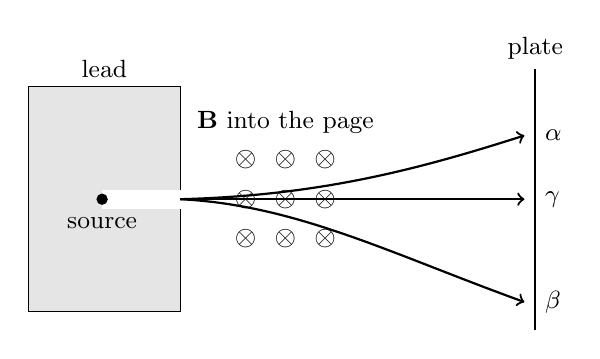
\begin{tikzpicture}[scale=0.92]
\draw[fill=gray!20] (0,-1.55) rectangle (2.1,1.55);
\draw[fill=white,draw=none] (1.02,-0.13) rectangle (2.12,0.13);
\draw[fill=black] (1.02,0) circle (0.07);
\node[below] at (1.02,-0.12) {\small source};
\node[above] at (1.05,1.55) {\small lead};
\foreach \x in {3.0,3.55,4.1}
  \foreach \y in {-0.55,0,0.55}
    \node at (\x,\y) {\(\otimes\)};
\node[above] at (3.55,0.78) {\small \(\mathbf B\) into the page};
\draw[thick] (7,-1.8) -- (7,1.8);
\node[above] at (7,1.8) {\small plate};
\draw[thick,->] (2.1,0) -- (6.85,0);
\draw[thick,->] (2.1,0) .. controls (4.0,0.05) and (5.35,0.40) .. (6.85,0.88);
\draw[thick,->] (2.1,0) .. controls (3.7,-0.08) and (5.0,-0.75) .. (6.85,-1.42);
\node[right] at (7,0.88) {\small \(\alpha\)};
\node[right] at (7,0) {\small \(\gamma\)};
\node[right] at (7,-1.42) {\small \(\beta\)};
\end{tikzpicture}\caption{Ein gebündelter radioaktiver Strahl in einem transversalen Magnetfeld. Die neutrale Komponente wird nicht abgelenkt, während sich die entgegengesetzt geladenen Komponenten in entgegengesetzte Richtungen und unterschiedlich stark krümmen.}\end{figure}

Die drei Komponenten erhielten die Namen Alpha, Beta und Gamma. In moderner Terminologie gilt:
\begin{equation}
\begin{aligned}
\beta\text{-radiation} &= \text{electrons},\\
\alpha\text{-radiation} &= \text{helium nuclei},\\
\gamma\text{-radiation} &= \text{photons}.
\end{aligned}
\end{equation}
Ein Alphateilchen enthält zwei Protonen und zwei Neutronen, was seine Massenzahl vier erklärt. In Daltons näherungsweise ganzzahliger Folge hätte Helium daher die Nummer vier eingenommen: vier nukleare Masseneinheiten auf Wasserstoffbasis. Betastrahlen sind die negativ geladenen Elektronen, die bereits aus Kathodenstrahlversuchen bekannt waren. Gammastrahlen tragen keine elektrische Ladung.

Verwendet man eine ausreichend schwache Quelle und einen Detektor, der einzelne Ankünfte auflösen kann, wird aus der kontinuierlich wirkenden Belichtung eine Folge einzelner Ereignisse: Blip, Blip, Blip. Dasselbe lässt sich für Beta-, Alpha- und Gammastrahlung tun. Ein Geigerzähler vermittelt das richtige Bild, unabhängig davon, ob die frühesten Apparaturen genau in diesem Betriebsbereich verwendet wurden. Jede Komponente trifft in diskreten Bündeln ein. Gamma bleibt das Rätsel: Die Strahlung ist neutral, wird aber dennoch Ereignis für Ereignis nachgewiesen. Gammastrahlung ist Licht sehr hoher Energie, und Planck, insbesondere aber Einstein, brachten Licht mit Quanten in Verbindung. Bevor wir uns dieser Schlussfolgerung zuwenden, müssen wir jedoch die klassischen Hinweise auf den Wellencharakter des Lichts ernst nehmen.

\section{Der klassische Wellencharakter des Lichts}

Klassisch betrachtet war Licht das deutlichste Beispiel für Kontinuität. Es besteht aus elektrischen und magnetischen Feldern, die sich als kontinuierliche Wellen ausbreiten. Newton hatte ein Korpuskularbild bevorzugt, doch Wellenexperimente verdrängten es. Eine beschleunigte Ladung erzeugt elektromagnetische Strahlung. Eine makroskopische Antenne kann Radiowellen, Mikrowellen, Infrarotstrahlung, sichtbares Licht oder ultraviolette Strahlung aussenden; auch eine Ladung, die sich innerhalb eines Atoms bewegt, wirkt wie eine Antenne. Die ausgesandte Strahlung kann eine fotografische Platte belichten.

Ein einzelner Spalt liefert einen ersten Hinweis auf das Wellenverhalten. Wäre Licht ein Strom von Geschossen, würde man erwarten, dass ein schmaler Spalt einen scharf gebündelten Fleck erzeugt. Stattdessen breitet sich die Beleuchtung zu einem unscharfen Bereich aus. Die Ausbreitung allein ist jedoch kein schlüssiger Beweis, denn man könnte sich vorstellen, dass Teilchen durch Kräfte am Rand der Öffnung abgelenkt werden.

Zwei Öffnungen liefern den aussagekräftigeren Test. Zwei voneinander unabhängige Teilchenströme ergäben zwei überlappende verwaschene Bereiche, die vielleicht dort am hellsten wären, wo sie sich überlagern. Wellen verhalten sich anders. Ein Wellenberg aus der einen Öffnung kann auf einen Wellenberg aus der anderen treffen und sie verstärken; ein Wellenberg kann aber auch auf ein Wellental treffen und sich mit ihm auslöschen. Der Schirm zeigt daher abwechselnd helle und dunkle Streifen, darunter dunkle Stellen, die bei nur einer Öffnung beleuchtet würden.\footnote{Die schematische Darstellung rekonstruiert die Spalt- und Interferenzdiagramme, die im Vorlesungsvideo zwischen 00:25:00 und 00:29:49 entwickelt wurden.}

\begin{figure}[h]\centering
\resizebox{\linewidth}{!}{%
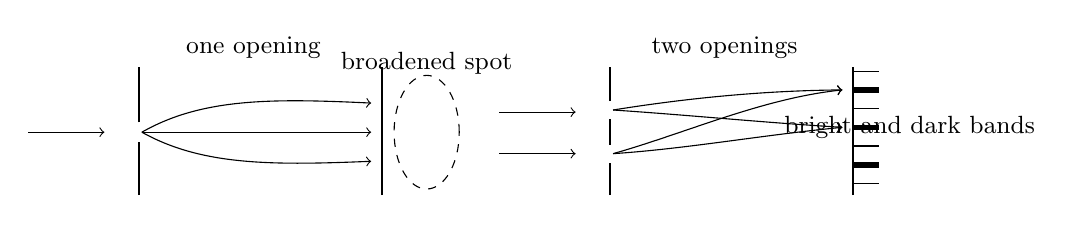
\begin{tikzpicture}[scale=0.88]
\begin{scope}
\draw[->] (-0.3,1.06) -- (0.8,1.06);
\draw[thick] (1.3,0.15) -- (1.3,0.92);
\draw[thick] (1.3,1.20) -- (1.3,2.0);
\draw[thick] (4.8,0.15) -- (4.8,2.0);
\draw[->] (1.34,1.06) .. controls (2.2,1.55) and (3.2,1.55) .. (4.65,1.48);
\draw[->] (1.34,1.06) -- (4.65,1.06);
\draw[->] (1.34,1.06) .. controls (2.2,0.58) and (3.2,0.58) .. (4.65,0.64);
\draw[dashed] (5.45,1.06) ellipse (0.47 and 0.82);
\node at (2.95,2.28) {\small one opening};
\node at (5.45,2.05) {\small broadened spot};
\end{scope}
\begin{scope}[xshift=6.8cm]
\draw[->] (-0.3,1.35) -- (0.8,1.35);
\draw[->] (-0.3,0.75) -- (0.8,0.75);
\draw[thick] (1.3,0.15) -- (1.3,0.62);
\draw[thick] (1.3,0.88) -- (1.3,1.25);
\draw[thick] (1.3,1.51) -- (1.3,2.0);
\draw[thick] (4.8,0.15) -- (4.8,2.0);
\draw[thin] (4.8,0.32) -- (5.18,0.32);
\draw[line width=2pt] (4.8,0.59) -- (5.18,0.59);
\draw[thin] (4.8,0.86) -- (5.18,0.86);
\draw[line width=2pt] (4.8,1.13) -- (5.18,1.13);
\draw[thin] (4.8,1.40) -- (5.18,1.40);
\draw[line width=2pt] (4.8,1.67) -- (5.18,1.67);
\draw[thin] (4.8,1.94) -- (5.18,1.94);
\draw[->] (1.34,0.75) .. controls (2.4,0.82) and (3.5,1.02) .. (4.65,1.13);
\draw[->] (1.34,1.38) .. controls (2.4,1.31) and (3.5,1.20) .. (4.65,1.13);
\draw[->] (1.34,0.75) .. controls (2.4,1.05) and (3.5,1.55) .. (4.65,1.67);
\draw[->] (1.34,1.38) .. controls (2.4,1.55) and (3.5,1.66) .. (4.65,1.67);
\node at (2.95,2.28) {\small two openings};
\node at (5.62,1.13) {\small bright and dark bands};
\end{scope}
\end{tikzpicture}}\caption{Ein einzelner Spalt erzeugt ein verbreitertes Bild, während zwei Spalte abwechselnd konstruktive und destruktive Interferenz hervorrufen.}\end{figure}

Denselben Effekt kann man sich mit Wasser leicht vorstellen. Bewegt man zwei Finger in der Wasseroberfläche, breiten sich kreisförmige Wellen aus, verstärken sich an manchen Stellen und löschen sich an anderen aus. Interferenz ist das entscheidende Kennzeichen einer Welle, nicht bloße Ausbreitung.

Auch hier ist die historische Abfolge nicht einfach. In dieser schematischen Darstellung steht Huygens vor Newton als Vertreter der Wellenausbreitung; Thomas Young wird mit dem Interferenznachweis in Verbindung gebracht, und einige optische Experimente Newtons lassen sich als Welleninterferenz deuten, obwohl er Korpuskeln bevorzugte. Die späteren Interferenzexperimente begründeten den Wellencharakter des Lichts über jeden vernünftigen Zweifel hinaus.

Maxwell identifizierte dann, was schwingt. Breitet sich eine Lichtwelle entlang einer Achse aus, steht ihr elektrisches Feld quer zu dieser Achse. Auch ihr magnetisches Feld steht quer zur Ausbreitungsrichtung und senkrecht zum elektrischen Feld. Das vollständige Muster breitet sich mit Lichtgeschwindigkeit aus.\footnote{Die schematische Darstellung rekonstruiert das Diagramm der elektromagnetischen Welle, das im Vorlesungsvideo bei 00:31:08 gezeichnet wurde.}

\begin{figure}[h]\centering
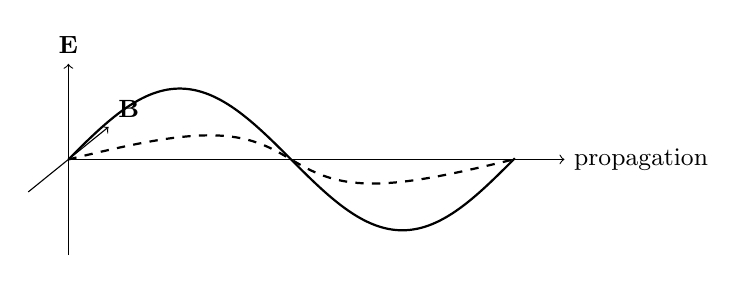
\begin{tikzpicture}[
  scale=0.9,
  x={(1cm,0cm)},
  y={(0cm,1cm)},
  z={(0.42cm,0.34cm)}
]
\draw[->] (0,0,0) -- (7,0,0) node[right] {\small propagation};
\draw[->] (0,-1.35,0) -- (0,1.35,0) node[above] {\small \(\mathbf E\)};
\draw[->] (0,0,-1.35) -- (0,0,1.35) node[above right] {\small \(\mathbf B\)};
\draw[thick,smooth,variable=\x,domain=0:6.3,samples=100]
  plot ({\x},{sin(\x r)},0);
\draw[thick,dashed,smooth,variable=\x,domain=0:6.3,samples=100]
  plot ({\x},0,{sin(\x r)});
\end{tikzpicture}\caption{In einer elektromagnetischen Welle stehen das elektrische und das magnetische Feld senkrecht aufeinander; beide sind transversal zur Ausbreitungsrichtung.}\end{figure}

Gewöhnliches sichtbares Licht schwingt viel zu schnell, als dass sich die wechselnden Felder direkt verfolgen ließen. Bei einer extrem langen Radiowelle wäre die Schwingung entsprechend langsamer. In beiden Fällen führt dieselbe Geometrie einer Transversalwelle zu Interferenz.

\section{Wellenlänge, Periode und Frequenz}

Die Wellenlänge \(\lambda\) ist eine räumliche Strecke: Man beginnt an einem Punkt der Schwingung und bewegt sich entlang der Welle, bis nach einem vollständigen Zyklus dieselbe Phase wiederkehrt. Sie wird in Metern, Zentimetern oder einer anderen Längeneinheit gemessen.

Bleibt man nun an einem Ort stehen, während die Welle vorbeiläuft, so ist die für einen vollständigen Zyklus benötigte Zeit die Periode \(T\). Sichtbares Licht hat eine extrem kurze Periode, ungefähr in der Größenordnung von \(10^{-15}\,\mathrm{s}\); eine größere Wellenlänge entspricht einer längeren Periode, eine kleinere Wellenlänge einer kürzeren Periode.

Während einer Periode legt eine Welle eine Wellenlänge zurück. Für eine Welle mit der Geschwindigkeit \(v\) gilt daher
\begin{equation}
v=\frac{\lambda}{T}.
\end{equation}
Wasser- und Schallwellen haben jeweils ihre eigene Ausbreitungsgeschwindigkeit. Für Licht gilt
\begin{equation}
c=\frac{\lambda}{T}.
\end{equation}
Die Frequenz \(f\) ist die Anzahl der Zyklen pro Zeiteinheit:
\begin{equation}
f=\frac{1}{T}.
\end{equation}
Also gilt
\begin{equation}
\lambda f=c.
\end{equation}
Wellenlänge und Frequenz bestimmen einander eindeutig.

\begin{figure}[h]\centering
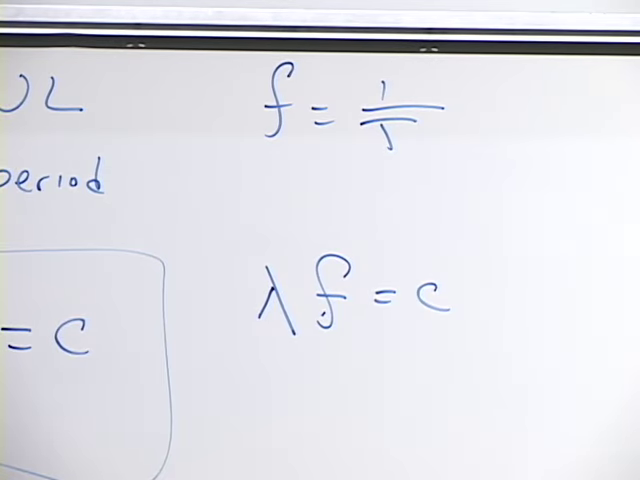
\includegraphics[width=0.68\textwidth]{lecture_01_figure_03.png}\caption{Für eine Lichtwelle gilt \(f=1/T\) und \(\lambda f=c\).}\lectureframe{00:36:24}\end{figure}

Physiker geben die Schwingungsrate oft in Radiant pro Sekunde statt in vollständigen Zyklen pro Sekunde an. Man stelle sich eine gleichförmige Bewegung auf einem Kreis vor. Führt der Punkt jede Sekunde \(f\) Umläufe aus und enthält jeder Umlauf \(2\pi\) Radiant, so ist seine Kreisfrequenz
\begin{equation}
\omega=2\pi f,
\qquad
\frac{\omega}{2\pi}=f.
\end{equation}
Vorerst ist dies eine Definition; auf die praktische Frage, ob dadurch die Anzahl der Faktoren \(2\pi\) sinkt, kommen wir später zurück.

Aus \(f=c/\lambda\) und \(\omega=2\pi f\) folgt
\begin{equation}
\omega=\frac{2\pi c}{\lambda},
\qquad
\omega\lambda=2\pi c.
\end{equation}
Bei einer anderen Wellenart tritt an die Stelle von \(c\) deren Ausbreitungsgeschwindigkeit.

\begin{figure}[h]\centering
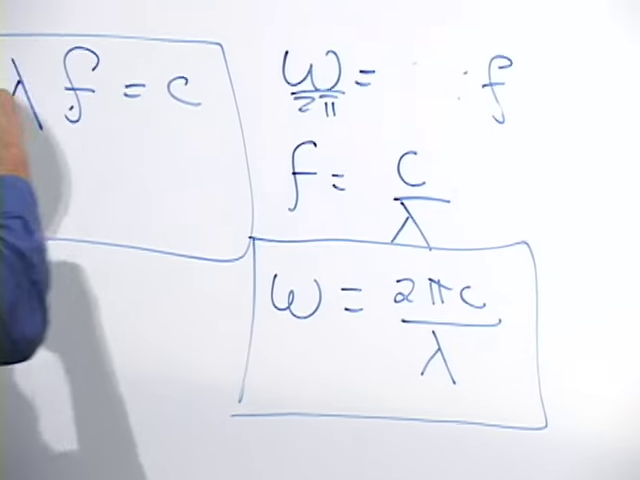
\includegraphics[width=0.68\textwidth]{lecture_01_figure_04.png}\caption{Für \(\omega=2\pi f\) gilt bei einer Lichtwelle \(\omega=2\pi c/\lambda\).}\lectureframe{00:39:10}\end{figure}

Elektromagnetische Strahlung bildet ein kontinuierliches Spektrum. In der üblichen Reihenfolge von längerer zu kürzerer Wellenlänge lauten die Bezeichnungen:
\begin{equation}
\begin{aligned}
\text{radio}
&\longrightarrow \text{microwave}
\longrightarrow \text{infrared}
\longrightarrow \text{visible}\\
&\longrightarrow \text{ultraviolet}
\longrightarrow \text{X ray}
\longrightarrow \text{gamma ray}.
\end{aligned}
\end{equation}
Sichtbares Licht nimmt nur einen schmalen Bereich ein. Die Grenzen zwischen den benannten Bereichen sind Konvention; hier benötigen wir daher keine exakten Grenzwellenlängen. Radiowellen können extrem lang sein; Gammastrahlung liegt am Ende des elektromagnetischen Spektrums mit den kürzesten Wellenlängen. Damit ist das Problem klar umrissen: Gammastrahlung ist klassisch eine kontinuierliche Feldwelle, wird aber in einzelnen Blips nachgewiesen.

\section{Diskrete Ankünfte und Wellenwahrscheinlichkeiten}

Thermodynamische Eigenschaften der Strahlung führten Planck und Einstein zu dem Schluss, dass Licht als diskrete Einheiten behandelt werden muss. Ein gedankliches Experiment veranschaulicht den Punkt, behauptet aber nicht, dass die Entdeckung tatsächlich auf diesem historischen Weg zustande kam.

Richtet man einen Strahl auf einen Schirm, erzeugt er bei gewöhnlicher Intensität einen zusammenhängend beleuchtet wirkenden Fleck. Setzt man einen teilweise lichtundurchlässigen Abschwächer in den Strahlengang, wird der Fleck dunkler. Erhöht man die Abschwächung wiederholt, trifft pro Zeiteinheit weniger Licht ein. Schließlich ändert sich das Erscheinungsbild. Statt eines kontinuierlich dunkler werdenden Flecks registriert der Detektor einzelne, isolierte Ereignisse.\footnote{Die schematische Darstellung rekonstruiert das Abschwächungsexperiment, das im Vorlesungsvideo zwischen 00:42:32 und 00:45:42 entwickelt wurde.}

\begin{figure}[h]\centering
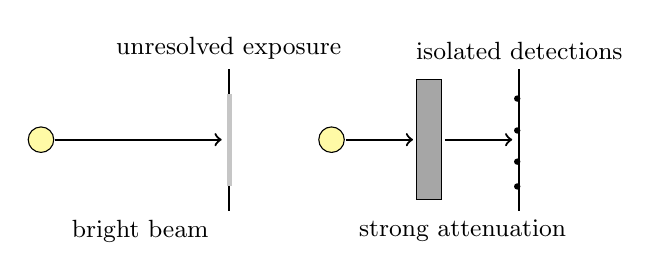
\begin{tikzpicture}[scale=0.9]
\begin{scope}
\draw[fill=yellow!35] (0,0) circle (0.18);
\draw[->,thick] (0.2,0) -- (2.55,0);
\draw[thick] (2.65,-1.0) -- (2.65,1.0);
\node[below] at (1.4,-1.0) {\small bright beam};
\end{scope}
\begin{scope}[xshift=4.1cm]
\draw[fill=yellow!35] (0,0) circle (0.18);
\draw[->,thick] (0.2,0) -- (1.15,0);
\draw[fill=gray!70] (1.2,-0.85) rectangle (1.55,0.85);
\draw[->,thick] (1.6,0) -- (2.55,0);
\draw[thick] (2.65,-1.0) -- (2.65,1.0);
\node[below] at (1.85,-1.0) {\small strong attenuation};
\end{scope}
\fill[gray!45] (2.62,-0.65) rectangle (2.70,0.65);
\foreach \y in {-0.66,-0.31,0.13,0.58}
  \fill (6.72,\y) circle (0.045);
\node[above] at (2.65,1.0) {\small unresolved exposure};
\node[above] at (6.75,1.0) {\small isolated detections};
\end{tikzpicture}\caption{Durch schrittweise Abschwächung sinkt die Nachweisrate, bis sich aus einer kontinuierlich wirkenden Belichtung einzelne Photonenereignisse auflösen lassen.}\end{figure}

Wartet man lange genug, summieren sich die Ereignisse zum selben räumlichen Profil wie der ursprüngliche Fleck. Der helle Bereich war also die nicht aufgelöste Summe vieler einzelner Ankünfte. Dieses Experiment mit geringer Intensität lässt sich durchführen, war aber nicht das frühe Experiment, das ursprünglich die Photonhypothese nahelegte. Einsteins Photonenvorschlag entstand aus thermodynamischen und photoelektrischen Überlegungen; das Abschwächungsexperiment veranschaulicht seine Konsequenz besonders direkt.

Setzt man nun zwei Spalte in den Strahlengang und verringert die Intensität, bis die Photonen einzeln eintreffen, ist jede Detektion ein lokalisierter Blip. Nach vielen Detektionen füllen die Blips jedoch ein Interferenzmuster mit hellen und dunklen Streifen aus. Die einzelnen Ankünfte sind zufällig, doch ihre Wahrscheinlichkeitsverteilung entspricht der vom Wellenmuster vorhergesagten Verteilung. Die klassische Welle ist zu einer Welle geworden, die Wahrscheinlichkeiten bestimmt.

Welle und Teilchen sind also nicht zwei getrennte Arten von Entitäten, die verschiedenen Bereichen der Natur zugeordnet werden. Sie sind zwei Erscheinungsformen desselben Quantenobjekts. Licht lässt sich weder allein als Welle noch allein als Teilchen angemessen beschreiben.

Bei Elektronen kehrt sich die ursprüngliche Überraschung um. Elektronen gelten als Teilchen und treffen einzeln auf einen Detektor, doch bei hinreichend eng benachbarten Spalten erzeugen auch sie ein Interferenzmuster. Alphateilchen, die etwa achttausendmal schwerer sind als Elektronen, folgen demselben Prinzip, auch wenn das Experiment schwieriger ist. Interferenz wurde sogar mit Buckyballs beobachtet: Molekülen aus sechzig Kohlenstoffatomen, die ungefähr wie ein verallgemeinerter Fußball angeordnet sind. Es wird erwartet, dass dasselbe Prinzip sogar für Bowlingkugeln gilt, auch wenn ein solches Experiment praktisch völlig undurchführbar ist. Die Diskussion lässt sich auf vorgeschlagene Experimente mit Viren oder lebenden Zellen als zunehmend ambitionierte Beispiele ausweiten. Um zu verstehen, wie Wellen- und Teilchenbeschreibungen zusammenpassen, braucht man Quantenmechanik; zunächst geht es darum, die für die Teilchenphysik benötigten Eigenschaften der Photonen herauszuarbeiten.

\section{Photonenenergie}

Photonen sind die diskreten, unteilbaren Bestandteile des Lichts. Licht transportiert Energie---Sonnenlicht erwärmt einen absorbierenden Gegenstand---, also muss jedes Photon Energie tragen. Eine monochromatische Welle hat eine bestimmte Wellenlänge und Kreisfrequenz, und jedes Photon in ihr besitzt
\begin{equation}
E_\gamma=\hbar\omega.
\end{equation}
Der Versuch, sich eine kontinuierliche Welle als kleine mechanische Ansammlung von Punkten vorzustellen, führt in die Irre. Fest steht die experimentelle Kombination: Lokalisierte Detektionen treten mit einer wellenbestimmten Verteilung auf, und die Energie trifft in unteilbaren Einheiten ein.

Da
\begin{equation}
\omega=\frac{2\pi c}{\lambda},
\end{equation}
eine kürzere Wellenlänge eine größere Kreisfrequenz und damit mehr Energie pro Photon bedeutet,
\begin{equation}
\lambda\downarrow
\quad\Longrightarrow\quad
\omega\uparrow
\quad\Longrightarrow\quad
E_\gamma\uparrow.
\end{equation}
hat ein einzelnes Radiophoton sehr wenig Energie. Ein Radiostrahl kann dennoch insgesamt sehr viel Energie transportieren, wenn er sehr viele Photonen enthält. Für einen monochromatischen Impuls mit \(n\) Photonen gilt
\begin{equation}
E_{\text{pulse}}=n\hbar\omega,
\qquad
n=0,1,2,\ldots.
\end{equation}
Die Gesamtenergie kann groß sein, bleibt aber ein ganzzahliges Vielfaches der Energie eines einzelnen Photons.

Diese Beziehung führt zu der praktischen Frage, die den weiteren Verlauf der Diskussion bestimmen wird. Warum muss man immer größere Maschinen bauen, um immer kleinere Dinge zu sehen? Warum nicht eine kleine Maschine für ein kleines Objekt verwenden? Die erste Hälfte der Antwort liegt bereits vor: Um kleinere Strukturen aufzulösen, braucht man eine kürzere Wellenlänge, und ein Quant kürzerer Wellenlänge trägt mehr Energie.

\section{Ruheenergie und invariante Masse}

Die Teilchenphysik verbindet Quantenmechanik mit Relativitätstheorie. Die Photonenbeziehung \(E_\gamma=\hbar\omega\) liefert den quantenmechanischen Teil; die entsprechende elementare Tatsache aus der Relativitätstheorie lautet
\begin{equation}
E_{\mathrm{rest}}=mc^2.
\end{equation}
Die Einschränkung ist wichtig. Ältere Darstellungen unterschieden zwischen der \emph{Ruhemasse} und der geschwindigkeitsabhängigen \emph{bewegten Masse}. In der modernen Terminologie bezeichnet \emph{Masse} die invariante Masse eines Objekts. Bewegung verändert seine Energie, nicht seine Masse. Jedes Elektron hat dieselbe Masse, unabhängig von seinem Bewegungszustand, während die Energie eines Elektrons bei seiner Beschleunigung zunimmt. In dieser Form ist \(E=mc^2\) also die Energie eines massiven Objekts in einem Bezugssystem, in dem das Objekt als Ganzes ruht.

Das Objekt muss nicht im Inneren bewegungslos sein. Ein Gaskasten kann auf einer Waage stillstehen, während seine Moleküle sich rasch in alle Richtungen bewegen. Die Energie dieser inneren Bewegungen gehört zur Ruheenergie des gesamten Kastens. Man beginnt mit einem kalten Kasten, misst seine Masse und fügt dann Wärmeenergie hinzu, während der Kasten selbst in Ruhe bleibt. Seine Ruhemasse ändert sich um
\begin{equation}
\Delta m=\frac{\Delta E_{\mathrm{internal}}}{c^2}.
\end{equation}
Sein Gewicht und seine Trägheit nehmen mit seiner Masse zu. Bei einem gewöhnlichen Kasten ist der Effekt selbst nach einer großen Temperaturerhöhung auf einer gewöhnlichen Waage viel zu klein, um ihn zu bemerken; die geringe Größe des Effekts ändert nichts am Prinzip.

Ein prägnanteres Beispiel sind ein Elektron und ein Positron. Sie haben exakt gleiche Massen und entgegengesetzte elektrische Ladungen. Sind sie zunächst in Ruhe und vernichten sie sich gegenseitig, tragen Photonen die Energie davon:
\begin{equation}
e^-+e^+\longrightarrow \text{photons}.
\end{equation}
Die anfängliche Energie beträgt
\begin{equation}
E_{\mathrm{initial}}=2m_e c^2,
\end{equation}
und diese Energie kann nicht verschwinden. Ein einzelnes Paar liefert nur eine winzige Energiemenge. Um auch nur eine Tasse Kaffee zu erwärmen, wären daher enorm viele Paare nötig; einzelne Vernichtungsereignisse zeigen die Umwandlung jedoch unmittelbar.

Für ein ruhendes Objekt sind Masse und Energie somit dieselbe physikalische Größe, ausgedrückt in unterschiedlichen Einheiten. Der Faktor \(c^2\) ist der Umrechnungsfaktor zwischen den gebräuchlichen Masse- und Energieeinheiten, ähnlich einem Zahlenfaktor zur Umrechnung von Metern in Zentimeter.

\begin{classroomqa}\lecturetimestamp{01:04:39}\audiencequestion{Erfordert die Umwandlung von Masse in freigesetzte Energie einen Mechanismus?}\lecturerresponse{Ja, dafür ist ein physikalischer Mechanismus erforderlich, doch Erhaltungssätze schränken das Ergebnis bereits ein. Selbst bevor der mikroskopische Vernichtungsmechanismus beschrieben wird, muss die anfängliche Energie von Elektron und Positron irgendwo wieder auftauchen. Die Energieerhaltung kann daher einen wichtigen Teil der Antwort bestimmen, ohne dass die Wechselwirkung im Einzelnen erklärt wird.--}\end{classroomqa}

\section{Dimensionen und die Wahl der Einheiten}

In SI-Einheiten ist die Lichtgeschwindigkeit eine sehr große Zahl und das Plancksche Wirkungsquantum eine sehr kleine. Dass Letzteres klein ist, legt bereits die Photonenbeziehung nahe: Die Kreisfrequenz sichtbaren Lichts ist enorm, während die Energie eines einzelnen Photons winzig ist. Daher muss \(E_\gamma=\hbar\omega\) in diesen Einheiten einen kleinen Zahlenwert von \(\hbar\) erfordern. In der Größenordnung gilt
\begin{equation}
c\sim 10^8\ \mathrm{m\,s^{-1}},
\qquad
\hbar\sim 10^{-34}\ \mathrm{J\,s}.
\end{equation}
\editorialnote{Beibehalten werden nur die in der Vorlesung angegebenen Größenordnungen, da die letzten Ziffern an der Tafel undeutlich sind.}
Einheiten sind unverzichtbar: Keine der beiden Konstanten ist einfach eine dimensionslose Dezimalzahl. Da die Energie die Dimensionen
\begin{equation}
[E]=M L^2 T^{-2},
\end{equation}
hat und \(E_\gamma=\hbar\omega\) mit \([\omega]=T^{-1}\) gilt, hat das Plancksche Wirkungsquantum die Dimensionen
\begin{equation}
[\hbar]=[E]T=M L^2 T^{-1}.
\end{equation}

Wenn man \(c\) groß und \(\hbar\) klein nennt, setzt man bereits eine Einheitenwahl voraus. Misst man die Geschwindigkeit in Fuß pro Stunde, erhält man für \(c\) einen anderen Zahlenwert als bei der Messung in Metern pro Sekunde. In Lichtjahren pro Jahr oder Lichtsekunden pro Sekunde beträgt die Lichtgeschwindigkeit einfach eins. Durch eine geeignete abgestimmte Wahl der Einheiten für Masse, Länge und Zeit lässt sich ebenso \(\hbar=1\) setzen.

Vertraute Einheitensysteme sind überlieferte Konventionen und keine privilegierten Merkmale der Natur. Eine Meile umfasst 5280 Fuß, ein Stone entspricht vierzehn Pfund, Pferde misst man in Hand, und Leistung kann in Pferdestärken angegeben werden. Das metrische System ist systematischer, doch auch seine Maßstäbe sind menschliche Festlegungen. Nichts in der fundamentalen Physik zeichnet Meter, Sekunde oder Kilogramm besonders aus.

Länge, Zeit und Masse liefern drei unabhängige grundlegende Einheiten:
\begin{equation}
L,\qquad T,\qquad M.
\end{equation}
Andere mechanische Einheiten lassen sich daraus bilden. Welche Wahl nützlich ist, hängt vom Problem ab. In der Astrophysik ist die Sonnenmasse praktisch; in der Kernphysik kann die Protonenmasse nützlich sein; Lichtjahre und Jahre machen relativistische astronomische Formeln kompakt. Mit drei unabhängigen Wahlmöglichkeiten lassen sich drei unabhängigen dimensionsbehafteten Konstanten zweckmäßige Zahlenwerte zuweisen. Astrophysik, Atomphysik und Teilchenphysik müssen nicht dieselben Einheiten wählen.

Für die Teilchenphysik sind zwei Konventionen besonders nützlich:
\begin{equation}
c=1,
\qquad
\hbar=1.
\end{equation}
Für die verbleibende Einheit gibt es keine vergleichbar ausgezeichnete Teilchenmasse. Man könnte die Protonenmasse, die Higgs-Boson-Masse oder die Myonenmasse gleich eins setzen, würde damit aber lediglich ein Mitglied einer großen Gruppe bevorzugen.

Warum also \(c\) und \(\hbar\) wählen? Eine erste Antwort könnte lauten, dass sie in vielen Gleichungen vorkommen. Das häufige Auftreten reicht nicht aus: Auch die Protonenmasse erscheint in vielen Gleichungen, ebenso die Größe des Protons. Was \(c\) und \(\hbar\) auszeichnet, ist ihre Universalität.

Die Konstanten \(c\) und \(\hbar\) sind verschieden. Die Geschwindigkeit \(c\) setzt jedem physikalischen Objekt eine Grenze: Massive Objekte können sich ihr annähern, aber nicht über sie hinaus beschleunigt werden. Das Plancksche Wirkungsquantum begrenzt jedes Quantenobjekt durch die Unschärferelation in der Größenordnung
\begin{equation}
\Delta x\,\Delta p\gtrsim\hbar.
\end{equation}
Keine der beiden Aussagen zeichnet eine bestimmte Teilchenart aus. Diese Universalität macht \(c=1\) und \(\hbar=1\) zu natürlichen Konventionen.

Das Proton liefert keine vergleichbare universelle Skala. Es ist nur ein Objekt unter vielen. Die Protonenmasse gleich eins zu setzen, hätte keinen fundamentaleren Status, als die Masse eines Rubidiumatoms gleich eins zu setzen; Elektron, Higgs-Boson und Myon werfen dasselbe Problem auf.

Die elektrische Ladung legt eine weitere universelle Größe nahe; nachdem \(c\) und \(\hbar\) jedoch normiert wurden, ist die physikalisch bedeutsame elektromagnetische Kopplung dimensionslos. Durch eine Änderung der Einheiten lassen sich dimensionsbehaftete Konstanten in einer elektromagnetischen Formel verschieben; eine echte dimensionslose Kopplung lässt sich dadurch nicht ändern.

Die Gravitation liefert eine dimensionsbehaftete universelle Konstante. In der Newtonschen Form lautet der Betrag der Kraft zwischen zwei Massen
\begin{equation}
F=G\frac{m_1m_2}{r^2}.
\end{equation}
Jede Masse gravitativ wechselwirkt, wohingegen elektrisch neutrale Objekte nicht an einer elektrischen Kraft beteiligt sein müssen. Damit besitzt \(G\) die erforderliche Universalität. Für die gewöhnliche Teilchenphysik ist sie dennoch eine unpraktische Normierung, da die Gravitationskräfte zwischen bekannten Elementarteilchen in den hier betrachteten Rechnungen vernachlässigbar sind.

\begin{classroomqa}
\lecturetimestamp{01:20:34}
\audiencequestion{Ist es gerechtfertigt, \(G\) einfach außer Acht zu lassen? Bei sehr hohen Energien verhalten sich Elementarteilchen möglicherweise nicht gemäß der klassischen Gravitation, wie hier angenommen.}
\lecturerresponse{Einzelne Teilchen reagieren auf das Gravitationsfeld der Erde: Ein einzelnes Teilchen fällt in diesem Feld. Der Gravitationseinfluss eines Elementarteilchens auf ein anderes wurde nicht direkt gemessen; daher kann die Annahme der Universalität auf dieser Ebene infrage gestellt werden. Der unmittelbare Grund, \(G\) nicht zu berücksichtigen, ist praktischer, nicht grundsätzlicher Art: In gewöhnlichen teilchenphysikalischen Experimenten und Gleichungen ist der Beitrag der Gravitation vernachlässigbar klein.}
\end{classroomqa}

\begin{classroomqa}
\lecturetimestamp{01:22:01}
\audiencequestion{Könnte man statt der Gravitation die elektrische Wechselwirkung als dritte Konvention zur Festlegung der Einheiten verwenden?}
\lecturerresponse{Ja. Man kann elektromagnetische Einheiten wählen, in denen die elektrische Ladung oder die in Coulombs Gesetz auftretende Konstante normiert ist. Solche Konventionen werden verwendet. Elektronen stoßen einander ab, statt sich anzuziehen, doch dieses Vorzeichen steht einer solchen Wahl nicht entgegen. Hier wird diese Konvention lediglich nicht verwendet.}
\end{classroomqa}

\begin{classroomqa}
\lecturetimestamp{01:23:06}
\audiencequestion{Ist die elektrische Ladung dimensionslos, wenn \(c\) und \(\hbar\) gleich eins gesetzt werden?}
\lecturerresponse{Ja. Eine dimensionslose Größe, die mit dem Quadrat der elektrischen Ladung zusammenhängt, beträgt ungefähr \(1/137\). Die genaue Konvention und die Bedeutung dieser Zahl können zunächst zurückgestellt werden; hier kommt es darauf an, dass sie dimensionslos ist.}
\end{classroomqa}

\begin{classroomqa}
\lecturetimestamp{01:23:37}
\audiencequestion{Könnte man die Coulomb-Konstante als dritte Konstante wählen, die gleich eins gesetzt wird?}
\lecturerresponse{Sie lässt sich in die Konvention für elektromagnetische Einheiten aufnehmen. Damit kann die dimensionslose Kopplung \(1/137\) nicht auf eins gebracht werden, denn eine Änderung der Einheiten kann eine dimensionslose Zahl nicht verändern. Es wird kein besonderer Vorteil dafür beansprucht, hier diese Konvention zu verwenden.}
\end{classroomqa}

\section{Gleichungen in natürlichen Einheiten und Bezugssysteme}

Mit \(c=1\) nimmt die Ruheenergiebeziehung für ein massives Objekt die Form an
\begin{equation}
E_{\mathrm{rest}}=m.
\end{equation}
Mit \(\hbar=1\) nimmt die Beziehung für das Photon die Form an
\begin{equation}
E_\gamma=\omega.
\end{equation}
Die Konstanten können jederzeit wieder eingesetzt werden, wenn numerische Größen in konventionellen Einheiten benötigt werden.

\begin{figure}[h]
\centering
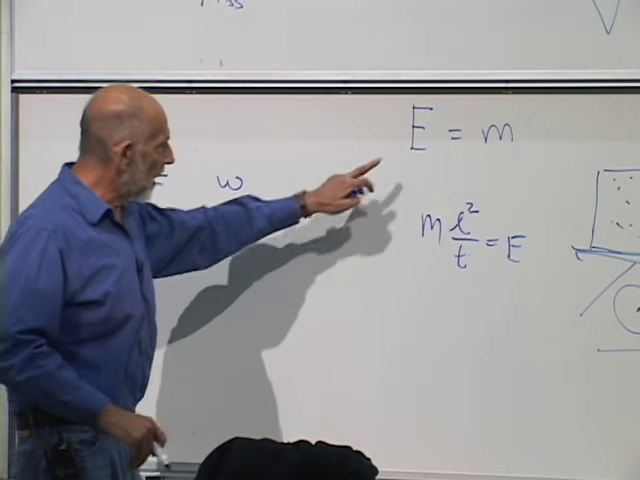
\includegraphics[width=0.72\textwidth]{lecture_01_figure_05.png}
\caption{In Einheiten mit \(c=1\) beträgt die Ruheenergie eines ruhenden massiven Objekts \(E=m\).}
\lectureframe{01:25:40}
\end{figure}

Diese Formeln sehen ähnlich aus, bedeuten aber Verschiedenes. In \(E_{\mathrm{rest}}=m\) ist \(E\) die Ruheenergie eines massiven Objekts. Ein Photon hat keine Masse und kann nicht in einen Ruhezustand gebracht werden; seine Energie ist daher keine Ruheenergie. Die Beziehung \(E_\gamma=\omega\) gibt die Energie eines bewegten, masselosen Quants an.

\begin{classroomqa}
\lecturetimestamp{01:26:07}
\audiencequestion{Was bedeutet \emph{in Ruhe}, wenn Ruhe immer relativ zu etwas ist und das Labor selbst nicht absolut ruht?}
\lecturerresponse{Ruhe wird relativ zu einem gewählten Bezugssystem definiert. Ist eine Tasse relativ zum Labor unbewegt, so ist ihre Energie in diesem Laborsystem ihre Masse, wenn \(c=1\); ein Beitrag aus einer Gesamtbewegung kommt dann nicht hinzu. Ein anderer Beobachter, der sich an der Tasse vorbeibewegt, schreibt ihr zusätzlich kinetische Energie zu. Verschiedene Beobachter ordnen demselben Objekt oder Photon im Allgemeinen unterschiedliche Energien zu: Energie ist bezugssystemabhängig, und die Annahme einer absoluten Ruhe ist nicht erforderlich.}
\end{classroomqa}

Die Konvention für die Kreisfrequenz lässt sich nun erneut betrachten. Die Schreibweise \(E_\gamma=\hbar\omega\) ist kompakt, doch \(\omega=2\pi f\) wurde zuvor ein Faktor \(2\pi\) eingeführt.

\begin{classroomqa}
\lecturetimestamp{01:28:13}
\audiencequestion{Warum verwendet man die Kreisfrequenz \(\omega\), gemessen in Radiant pro Sekunde, statt der scheinbar einfacheren Anzahl vollständiger Schwingungen pro Sekunde?}
\lecturerresponse{Die Wahl ist zum Teil historisch bedingt; die mathematische Antwort ist pragmatisch und nicht unmittelbar ersichtlich. Die hier vorgeschlagene Antwort ist vorläufig: Man schreibt die betreffenden Gleichungen einmal mit \(f\) und einmal mit \(\omega\) auf und prüft dann, bei welcher Konvention weniger Faktoren \(2\pi\) auftreten. Die Faktoren \(2\pi\) lassen sich nicht überall zugleich zum Verschwinden bringen. Außerdem wurde ein möglicher Zusammenhang mit der Schreibweise mithilfe komplexer Exponentialfunktionen angedeutet, hier aber nicht weiter ausgeführt.}
\end{classroomqa}

\begin{classroomqa}
\lecturetimestamp{01:29:51}
\audiencequestion{Kann man zwei Teilchen so weit beschleunigen, dass ihre gegenseitige Gravitationswechselwirkung wichtig wird?}
\lecturerresponse{Prinzipiell ja. In der Praxis sind heutige Beschleuniger von diesem Bereich außerordentlich weit entfernt. Die Antwort hängt auch davon ab, was mit einem Teilchen gemeint ist: Ein makroskopischer, gravitierender Körper ist nicht der hier betrachtete Fall eines Elementarteilchens.}
\end{classroomqa}

\begin{classroomqa}
\lecturetimestamp{01:30:27}
\audiencequestion{Was kann als Quelle für Positronen dienen?}
\lecturerresponse{Bei hochenergetischen Kollisionen können Positronen entstehen. Auch einige Kernprozesse und Zerfälle erzeugen sie.}
\end{classroomqa}

\begin{classroomqa}
\lecturetimestamp{01:30:53}
\audiencequestion{Sind die Planck-Zeit und die Planck-Länge die hier verwendeten natürlichen Einheiten?}
\lecturerresponse{Nein. Planck-Einheiten ergeben sich, wenn \(G\), \(c\) und \(\hbar\) alle gleich eins gesetzt werden. Die so erhaltene Planck-Länge ist viel kleiner als die Längenskalen der gewöhnlichen Teilchenphysik und daher hier ein unpraktisches Maß. Solche Einheiten sind dann natürlich, wenn Gravitation, Quantenmechanik und Relativität zugleich eine Rolle spielen, etwa in der Physik Schwarzer Löcher, der Kosmologie oder der Quantengravitation. Ist die Gravitation vernachlässigbar, ist es nützlicher, nur \(c\) und \(\hbar\) gleich eins zu setzen.}
\end{classroomqa}

\section{Impuls, Licht und Auflösungsvermögen}

Der nächste Grundbegriff ist der Impuls. Ein ruhendes Objekt hat keinen Impuls, obwohl es die von null verschiedene Ruheenergie \(mc^2\) besitzt. Sobald es sich bewegt, hat es im Allgemeinen Impuls. Bei einer Kollision ist der Impuls ebenso erhalten wie die Energie: Der gesamte Vektorimpuls ist vor und nach dem Zusammenstoß zweier Objekte gleich. Alles, was einem Erhaltungssatz unterliegt, verdient besondere Aufmerksamkeit.

Der Impuls ist ein Vektor: Er zeigt in Bewegungsrichtung. Für ein nichtrelativistisches Objekt gilt
\begin{equation}
\mathbf p=m\mathbf v.
\end{equation}
Dies ist nicht die allgemeine relativistische Formel und lässt sich nicht unmittelbar auf Licht anwenden.

Dennoch trägt Licht sowohl Impuls als auch Energie. Gewöhnliches Licht übt nur einen so kleinen Schub aus, dass sein Impuls schwer zu bemerken ist; ein intensiver Laserpuls kann jedoch einen beträchtlichen Impuls übertragen. Der große Laser in Livermore kann zum Beispiel Materie durch den von seiner Strahlung getragenen Impuls nach innen treiben.

Betrachten wir einen Puls, dessen Strahlen so gut gebündelt sind, dass sie sich nahezu entlang einer Achse bewegen. Ein realer Strahl kann eine gewisse Winkeldivergenz aufweisen, sodass sich Teile davon in leicht unterschiedlichen Richtungen ausbreiten. Für einen ideal gebündelten Strahl zeigt der Impuls jedoch entlang des Strahls und hat den Betrag
\begin{equation}
p=\frac{E}{c},
\qquad\text{or equivalently}\qquad
E=cp.
\end{equation}
Diese Beziehung wird hier als relativistische Tatsache angenommen und nicht hergeleitet. Die folgende Dimensionsprüfung bestätigt lediglich, dass ihre Einheiten mit denen des gewöhnlichen Impulses übereinstimmen:
\begin{equation}
\left[\frac{E}{c}\right]
=
\frac{M L^2 T^{-2}}{L T^{-1}}
=
M L T^{-1}
=
[m v]
=
[p].
\end{equation}
Dieser Dimensionsvergleich schreibt dem Licht keine Ruhemasse zu. Ein Photon hat die Masse null; es trägt Impuls, weil es Energie trägt und sich mit \(c\) bewegt.

Die Richtung von \(\mathbf p\) ist die Ausbreitungsrichtung. Sein Betrag ist gewöhnlich schwer nachzuweisen, weil \(c\) im Nenner steht. Ein Strahl kann seine Energie leicht dadurch zeigen, dass er Materie erhitzt oder verdampft, während sein mechanischer Schub viel kleiner ist. Bei hinreichend großer Intensität kann dieser Schub jedoch erheblich werden.

Für ein Photon gilt
\begin{align}
p_\gamma
&=\frac{E_\gamma}{c}\\
&=\frac{\hbar\omega}{c}.
\end{align}
Um dies durch die Wellenlänge auszudrücken, betrachten wir die Wellenbeziehungen noch einmal sorgfältig. Da
\begin{equation}
f\lambda=c,
\qquad
\omega=2\pi f,
\end{equation}
lautet die korrekte Beziehung
\begin{equation}
\omega\lambda=2\pi c,
\qquad
\omega=\frac{2\pi c}{\lambda}.
\end{equation}
Der Faktor \(2\pi\) lässt sich leicht vertauschen, wenn man die Definitionen nicht ausschreibt. Setzt man erneut bei \(f\lambda=c\) und \(f=\omega/(2\pi)\) an, ist die Frage geklärt:
\begin{equation}
\frac{\omega}{2\pi}\lambda=c
\quad\Longrightarrow\quad
\omega\lambda=2\pi c.
\end{equation}
Einsetzen ergibt nun
\begin{align}
p_\gamma
&=\frac{\hbar}{c}\frac{2\pi c}{\lambda}\\
&=\frac{2\pi\hbar}{\lambda}\\
&=\frac{h}{\lambda}.
\end{align}

\begin{classroomqa}
\lecturetimestamp{01:42:38}
\audiencequestion{Ist \(2\pi\hbar\) gleich \(h\)?}
\lecturerresponse{Ja. Per Definition gilt \(h=2\pi\hbar\); somit ist \(p_\gamma=2\pi\hbar/\lambda\) dasselbe wie \(p_\gamma=h/\lambda\). Unabhängig davon, welche Frequenzkonvention gewählt wird, treten Faktoren \(2\pi\) irgendwo wieder auf.}
\end{classroomqa}

Je kürzer die Wellenlänge, desto größer der Impuls des Photons. Ein Radiophoton hat eine sehr lange Wellenlänge und einen winzigen Impuls. Ein Gammaphoton hat eine sehr kurze Wellenlänge und überträgt einen viel stärkeren Stoß. Ein einzelnes Photon bewirkt makroskopisch weiterhin nur einen kleinen Impuls, doch sein Impuls ist viel größer als der eines Radiophotons. Auch seine Energie ist größer, denn \(E_\gamma=cp_\gamma\).

Dieser Zusammenhang erklärt, warum kleinere Objekte größere Maschinen erfordern. Ein Foto, das mit Wellenlängen aufgenommen wird, die viel größer als ein menschlicher Kopf sind, könnte nur eine unscharfe Silhouette zeigen. Um Gesichtszüge zu unterscheiden, muss die Wellenlänge kürzer als der Kopf sein. Um ein einzelnes Haar aufzulösen, muss sie mit dessen Dicke vergleichbar oder kleiner sein. Um die Struktur eines Atoms aufzulösen, darf die Wellenlänge der Sonde nicht größer als das Atom sein:
\begin{equation}
\lambda_{\mathrm{probe}}\lesssim
\text{size of the structure to be resolved}.
\end{equation}
Für kleinere Strukturen braucht man also kürzere Wellenlängen, und kürzere Wellenlängen erfordern größeren Impuls und höhere Energie. Die Sonde muss kein Photon sein; auch hochenergetische Teilchen anderer Art folgen demselben quantenmechanischen Zusammenhang zwischen Wellenlänge und Impuls. Zu ihrer Erzeugung braucht man Beschleuniger, die jedem Teilchen mehr und mehr Energie übertragen. Das Paar \(p_\gamma=h/\lambda\) und \(E_\gamma=\hbar\omega\) trägt die Argumentation: Eine höhere Sondenenergie erhöht den Impuls und verkürzt die Wellenlänge.

Seit ungefähr einem Jahrhundert wiederholt sich in der Teilchenphysik dasselbe Muster: höhere Energie, größerer Impuls, kürzere Wellenlänge und feinere räumliche Auflösung.

\begin{classroomqa}
\lecturetimestamp{01:46:57}
\audiencequestion{Gibt es eine theoretische untere Grenze für die Wellenlänge?}
\lecturerresponse{Möglicherweise. In der Nähe der Planck-Länge wird etwas Neues erwartet, doch diese Antwort ist vorläufig. Falls die räumliche Auflösung dort an eine Grenze stößt, liegt diese Skala immer noch etwa siebzehn Größenordnungen unter den Abständen, die am LHC untersucht werden. Heutige Experimente sind also enorm weit davon entfernt.}
\end{classroomqa}

Dieselbe Argumentation legt einen groben Zusammenhang zwischen der Größe eines Beschleunigers und der Skala nahe, die er auflösen kann.

\begin{classroomqa}
\lecturetimestamp{01:48:02}
\audiencequestion{Hängen die Wellenlänge oder die Größe der aufgelösten Struktur ungefähr umgekehrt mit der Größe des Beschleunigers zusammen?}
\lecturerresponse{Ungefähr ja, sofern die maximalen elektrischen Felder zur Beschleunigung der Teilchen und die Magnetfelder zu ihrer Führung durch die verfügbaren Anlagen vorgegeben bleiben. Ein Beschleunigungsgradient ist ein Energiegewinn pro Längeneinheit. Für einen Linearbeschleuniger der Länge \(L\) und mit annähernd konstantem Gradient \(\mathcal G\) gilt
\[
E_{\mathrm{beam}}\sim \mathcal G L.
\]
Bei ultrarelativistischen Energien ist die auflösbare Wellenlänge umgekehrt proportional zur Energie. Eine Vergrößerung der Länge des Linearbeschleunigers verbessert daher die Auflösung ungefähr um den umgekehrten Faktor. Dies ist nur eine heuristische Skalierung, kein exaktes Gesetz. In Kreisbeschleunigern kann dieselbe Anlage wiederholt durchlaufen werden; beim Ablenken strahlen beschleunigte Ladungen jedoch Energie ab.}
\end{classroomqa}

\begin{classroomqa}
\lecturetimestamp{01:49:47}
\audiencequestion{Wie groß müsste ein Beschleuniger sein, um die Planck-Länge zu erreichen?}
\lecturerresponse{Nach dieser groben Skalierung müsste er etwa siebzehn Größenordnungen länger sein als der Beschleuniger am CERN. Das wäre nicht so groß wie das Universum, aber ungefähr galaktischen Ausmaßes.}
\end{classroomqa}

\begin{classroomqa}
\lecturetimestamp{01:50:09}
\audiencequestion{Wie verhalten sich die Energien der höchstenergetischen kosmischen Strahlung zu den Kollisionsenergien in Beschleunigern?}
\lecturerresponse{Einzelne kosmische Strahlungsteilchen können eine weitaus höhere Energie im Laborsystem haben. Für den Zahlenvergleich betrachten wir ein extremes kosmisches Strahlungsteilchen mit einer Laborenergie in der Größenordnung von \(10^{21}\,\mathrm{eV}=10^{12}\,\mathrm{GeV}\). Ein kosmisches Strahlungsteilchen trifft jedoch auf ein ruhendes Target im Labor, während in einem Beschleuniger zwei energiereiche Strahlen frontal aufeinanderprallen. Noch wichtiger ist, dass aussagekräftige Experimente eine hohe Teilchenflussrate benötigen: viele Teilchen und viele gut kontrollierte Kollisionen. Ein einzelnes kosmisches Strahlungsteilchen kann das relevante Target verfehlen oder ein Ereignis erzeugen, aus dem sich nur wenig erschließen lässt. Eine bewusst übertriebene Schätzung des Ölbedarfs setzte die Menge, die für den Betrieb eines brauchbaren galaktischen Beschleunigers nötig wäre, mit etwa hundert Billionen Barrel Öl pro Sekunde an. Sie soll zeigen, dass genügend Kollisionsstatistik mindestens ebenso große Schwierigkeiten bereiten würde wie die Länge des Beschleunigers.}
\end{classroomqa}

\editorialnote{Die Umrechnung des Ölbedarfs ist in der Quelle widersprüchlich. Zunächst wird der Wert genannt und dann mit etwa \(10^{14}\) Barrel pro Sekunde wiederholt; eine spätere erneute Angabe lautet \(10^{11}\) Barrel pro Sekunde. Beide Größenordnungen bleiben erhalten, statt den Widerspruch stillschweigend aufzulösen.}

Dies sind tatsächliche Abstände und nicht bloß formale Größen. Die praktische Frage lautet, wie man sie untersuchen kann, ohne einen galaktischen Beschleuniger zu bauen und seine fantastisch hohe Leistung bereitzustellen.

\begin{classroomqa}
\lecturetimestamp{01:52:55}
\audiencequestion{Wie ist die Energie am LHC mit einem kosmischen Strahlungsteilchen der Energie \(10^{12}\,\mathrm{GeV}\) zu vergleichen?}
\lecturerresponse{Für ein ultrarelativistisches Projektil mit Laborenergie \(E_{\mathrm{lab}}\), das auf ein ruhendes Target der Masse \(m_{\mathrm{target}}\) trifft, skaliert die Schwerpunktsenergie parametrisch wie folgt:
\[
E_{\mathrm{cm}}\simeq
\sqrt{2m_{\mathrm{target}}c^2E_{\mathrm{lab}}}.
\]
\editorialnote{Der angezeigte Ausdruck für ein ruhendes Target macht die in diesem Austausch genannte Quadratwurzel-Skalierung ausdrücklich sichtbar.}
Bei festgehaltener Targetmasse wächst die nutzbare Kollisionsenergie daher nur mit der Quadratwurzel der Projektilenergie. Ein kosmisches Strahlungsteilchen mit \(10^{12}\,\mathrm{GeV}\) entspricht somit größenordnungsmäßig kollidierenden Strahlen mit Energien von \(10^6\,\mathrm{GeV}\) pro Strahl, nicht \(10^{12}\,\mathrm{GeV}\) in jedem Strahl. Kosmische Strahlung kann die Energien irdischer Beschleuniger zwar übertreffen, doch wegen ihrer äußerst geringen Flussrate sind systematische, kontrollierte Experimente unpraktisch.}
\end{classroomqa}